\documentclass[11pt]{article}

\usepackage[a4paper, margin=1in]{geometry}
\usepackage{mathtools}
\usepackage{outlines}
\usepackage{amsmath}
\usepackage{pdfpages}
\usepackage{verbatim}
\usepackage{listings}
% \usepackage[dvipsnames]{xcolor}
\usepackage[english]{babel}
\usepackage[labelfont=bf]{caption}
\usepackage{hyperref}
\usepackage{subcaption}
\usepackage{array}
\usepackage{longtable}
%\usepackage[T1]{fontenc}
\usepackage{titlesec, blindtext, color}
\usepackage{float}
\usepackage{xcolor}
\pagecolor{white}
\definecolor{gray75}{gray}{0.75}
\newcommand{\hsp}{\hspace{10pt}}
\titleformat{\section}[hang]{\Huge\bfseries}{\thesection\hsp\textcolor{gray75}{|}\hsp}{0pt}{\Huge\bfseries}

\captionsetup{labelfont=bf}

\definecolor{codegreen}{rgb}{0,0.6,0}
\definecolor{codegray}{rgb}{0.5,0.5,0.5}
\definecolor{codepurple}{rgb}{0.58,0,0.82}
\definecolor{backcolour}{rgb}{0.95,0.95,0.95}


\lstdefinestyle{mystyle}{
    backgroundcolor=\color{backcolour},   
    commentstyle=\color{codegreen},
    keywordstyle=\color{blue},
    numberstyle=\tiny\color{codegray},
    stringstyle=\color{orange},
    basicstyle=\ttfamily\footnotesize,
    breakatwhitespace=false,         
    breaklines=true,                 
    captionpos=b,                    
    keepspaces=true,                 
    numbers=left,                    
    numbersep=5pt,                  
    showspaces=false,                
    showstringspaces=false,
    showtabs=false,                  
    tabsize=2
}

\lstset{style=mystyle}

\includeonly{
    chapters/introduction,
    chapters/pagerank,
    chapters/hadoop,
    chapters/spark-java,
    chapters/spark-python
}


\begin{document}
\begin{titlepage}
    \begin{center}
        \begin{figure}
            
\includegraphics[width=\textwidth]{img/marchio_unipi_pant541-eps-converted-to.pdf}         
        \end{figure}
        {\Large
        Artificial Intelligence and Data Engineering\\
        \vspace{5mm} %5mm vertical space
        Cloud Computing}\\
        \vspace{30mm} %5mm vertical space
        {\Huge\textbf{\textit{PageRank}}}\\
        \vspace{10mm} %5mm vertical space
        {\Large Project Documentation}\\
        \par\noindent\rule{\textwidth}{0.4pt}
            \begin{flushright}
                \textit{TEAM MEMBERS}:\\
                Daniele Cioffo\\
                Edoardo Fazzari\\ 
                Federica Baldi\\ 
                Mirco Ramo\\
        	
            \end{flushright}
            \vfill
        Academic Year: 2020/2021\\        
    \end{center}
\end{titlepage} 
   
\tableofcontents

\section{Introduction}

\subsection{Description}
Each chapter will contain a section describing the performance.

\section{PageRank}

\subsection{Introduction}
In this section a description of the MapReduce implementation of \textit{Page Rank} is given.
The algorithm is carried out in \textbf{four distinct steps}:
\begin{enumerate}
	\item \textit{Nodes counting} phase
	\item \textit{Graph Construction} phase
	\item \textit{Page Rank Computation} phase
	\item \textit{Sorting} phase
\end{enumerate}


\noindent We have decided to represent the structure of the graph through adjacency lists, so each node (that represents a page) will keep the list of outgoing edges as status information, as well as its ranking.



\subsection{First Phase: Nodes Counting}
To compute PageRank the total number of nodes is required. Considering that the number of nodes is unknown at the beginning –and may be huge–, this is assessed by using a MapReduce approach for optimization reasons.


\begin{algorithm}[H]
	\caption{Nodes Counter Mapper}\label{Mapper}
		\begin{algorithmic}[1]
			\Procedure{Map}{PageId id, Page p}
					\If {p is not empty}
						\State EMIT(uniqueKey, 1) 
					\EndIf
			\EndProcedure
	\end{algorithmic}
\end{algorithm}


\begin{algorithm}[H]
	\caption{Nodes Counter Reducer}\label{Reducer}
		\begin{algorithmic}[1]
			\Procedure{Reduce}{Key k, Values $[v_1, v_2, \dots]$}
					\ForAll {value \textbf{in} values}
						\State $sum \gets sum + value$
					\EndFor
					\State EMIT(N, sum)
			\EndProcedure
	\end{algorithmic}
\end{algorithm}


\subsection{Second Phase: Graph Construction}
In this phase we parse the information in the input file taking the information that interests us, i.e. the title of the page and the outgoing edges. Also, to each page, we provide the initial PageRank thanks to the already calculated total number of nodes. 

\begin{algorithm}[H]
	\caption{Graph Construction Mapper}\label{Mapper}
		\begin{algorithmic}[1]
			\Procedure{Map}{PageId id, Page p}
					\State $\textit{title} \gets \textit{getTitle(p)}$
					\State $ outgoingEdges \gets \textit{getOutgoingEdges(p)}$
		
					\State EMIT(title, outgoingEdges)
			\EndProcedure
			
			
	\end{algorithmic}
\end{algorithm}

\begin{algorithm}[H]
	\caption{Graph Construction Reducer}\label{Reducer}
		\begin{algorithmic}[1]
			\Procedure{InitReduce}{Configuration c}
				\State $N \gets c.numberOfNodes$
			\EndProcedure
		
			\Procedure{Reduce}{Title t, ListOfListOfEdges $[e_1, e_2, \dots]$}
					\State $\textit{initialPageRank} \gets \frac{1}{N} $
					\State $ \textit{edges} \gets e_1$
		
					\State EMIT(title, \{initialPageRank, edges\})
				
			\EndProcedure
		\end{algorithmic}
\end{algorithm}

\noindent In \textit{Algorithm 4} only $e_1$ is considered because the title is a unique identifier of the pages, so the list of input values will always consist of a single element. Only one mapper will manage one page.

\subsection{Third Phase: PageRank Estimation}
In this section, the relaxed pagerank iteration is presented.
\noindent The number of iteration is fixed at the start of the execution. We do not converge to a (or a more or less) consistent state, because the presence of dangling nodes will cause importance (i.e., pagerank mass) to leak out.

\begin{algorithm}
	\caption{PageRank Computation Mapper}\label{Mapper}
		\begin{algorithmic}[1]
						\Procedure{Map}{Key k, FormattedPage p}
			
			\State EMIT(p.title, \{0, p.outgoingEdges\})
			\ForAll{outgoingEdge \textbf{in} p.outgoingEdges}
			\State EMIT(outgoingEdge, $\{\frac{p.pagerank}{p.outgoingEdges.length}, NULL\}$)
			\EndFor
			\EndProcedure
	\end{algorithmic}
\end{algorithm}
Note: \textit{outgoingEdge} is a title itself.


\begin{algorithm}[H]
	\caption{PageRank Computation Reducer}\label{Reducer}
		\begin{algorithmic}[1]
			\Procedure{InitReduce}{Configuration c}
				\State $N \gets c.numberOfNodes$
				\State $D \gets Damping$
			\EndProcedure
		
			\Procedure{Reduce}{Title t, Nodes $[n_1, n_2, \dots]$}
				\If{title = DANGLING}
					\ForAll {node \textbf{in} nodes}
						\State $s \gets s + node.pagerank$	
					\EndFor
					\State EMIT(t, \{s, NULL\})
				\Else
					\State n \textbf{new} Node
					\ForAll {node \textbf{in} nodes}
						\If {node.hasOutgoingEdges()}
							\State n.outgoingEdges = node.outgoingEdges
						\Else
							\State $s = s + node.pagerank$
						\EndIf
					\EndFor
					\State$n.pagerank =  \frac{(1-D)}{N} + D*s$
					\State EMIT(t, n)
				\EndIf
			\EndProcedure
	\end{algorithmic}
\end{algorithm}



\subsection{Fourth Phase: Sorting}
The final step is sorting the webpages by decreasing rank, this is done making advantage of the sorting mechanism of MapReduce.

\begin{algorithm}[H]
	\caption{Sorting Mapper}\label{Mapper}
	\begin{algorithmic}[1]
		\Procedure{Map}{Key k, FormattedPage p}
		\State $title \gets p.title$
		\State $pagerank \gets p.pagerank$k
		\State EMIT(pagerank, title)
		\EndProcedure
	\end{algorithmic}
\end{algorithm}

\begin{algorithm}[H]
	\caption{Sorting Reducer}\label{Reducer}
	\begin{algorithmic}[1]
		\Procedure{Reduce}{Pagerank rank, Titles $[t_1, t_2, \dots]$}
		\ForAll {title \textbf{in} titles}
		\State EMIT(title, rank)
		\EndFor
		\EndProcedure
	\end{algorithmic}
\end{algorithm}

\section{Hadoop Implementation}
\subsection{Introduction}
In this section is briefly described how we have implemented in Hadoop the pseudocode presented in the previous chapter. After that, the performance evaluation of the computation is reported.

\subsection{First Phase: Graph construction}
Parsing is a job that doesn't need to create a conglomerate value, but it creates records which, each of them, is treated as a standalone piece of information. We decide to use three reducers since we have three working nodes.

\noindent Initially we had thought of inserting an initial step dedicated exclusively to the node count, but later we came up with a better solution, complicating the parsing phase. In the section on performance the differences between the two approaches will be shown, showing the improvement obtained.

\noindent First we consider the Mapper, in which each record is parsed, looking for the title and all the outgoing links. So for each record we are going to emit a pair \textbf{(title, outgoing edges)}. In addition to this we must also count the number of nodes, to do this we use an \textbf{In-Mapper Combiner}, a global counter inside the Mapper. It will be initialized to 0 in setup, and incremented at each execution of the map function; during the cleanup we will transmit a single cumulative value for that Mapper, transmitting the pair \textbf{("", N)}, with N the value of the counter. As a key we use the empty string "", which cannot belong to any title and which is always placed first in lexicographic order.
Since we send two different information between Mapper and Reducer, we have decided to implement our own \textbf{partitioner}, to always send partial counters to Reducer 0 and therefore be sure to have this value in the file part-r-00000. All other keys will be split into the other reducers, using an hash function, like the default behavior.
As for the reducer, it takes care of adding the partial values of the counters to obtain N, the number of nodes; in addition it will get the title and outgoing links values of each record. All this information will be saved in the filesystem, to be processed in the next step. The next step will take in input all the output file containing the Node information. All this process has been schematized in \ref{fig:parsingPhase}


\begin{figure}
	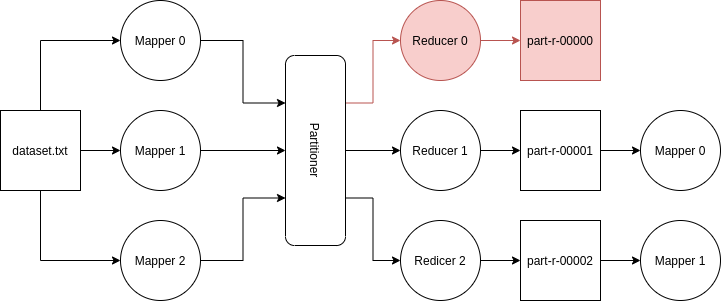
\includegraphics[width=\textwidth]{img/ParserSchema.png}
	\caption{Parsing phase}
	\label{fig:parsingPhase}     
\end{figure}

\subsection{Second Phase: PageRank Estimation}
Since the previous phase constructs multiple outputs, this phase has to take multiple inputs
As in the \textit{Graph construction} phase multiple reducers are used for accelerating the computation. Thus, from the first iteration to the last one this MapReduce computation takes multiple inputs and produces multiple outputs.

\subsection{Third Phase: Sorting}
Since the previous phase constructs multiple outputs, also this phase has to take multiple inputs. Here a single reducer is used in order to take advantage of the automatic sorting done over the keys by Hadoop. Keys are in this case the pagerank value of each page, and are passed by the mapper to the reducer as \textbf{DoubleWritable} objects. We have implemented a \textbf{WritableComparator} for getting the descending order.

\subsection{Performance}
For measuring the performance we considered three files with a different number of nodes:
\begin{itemize}
	\item \textbf{wiki-micro.txt}: number of nodes 2427. Most of the nodes points to sites that are not present in the initial set.
	\item \textbf{dataset5.txt}: number of nodes 5000. This dataset is synthetic dataset created using the same structure of \textit{wiki-micro.txt}. Each node has a random value of outgoing edges between 0 and 10.
	\item \textbf{dataset10.txt}: number of nodes 10000. This dataset is synthetic dataset created using the same structure of \textit{wiki-micro.txt}. Each node has a random value of outgoing edges between 0 and 10.
\end{itemize}
and we test them over different numbers of iteration: 5, 10, 15.

In order to prove the performance gain in \textit{In-Mapper Combiner} instead of counting the nodes in a MapReduce, we provide the result of both the approches.

\begin{table}[H]
\caption{Performance with MapReduce Node Counter}
\centering
\begin{tabular}{c c c c}
\hline\hline
File & N Iter 5 & N Iter 10 & N Iter 15 \\ [0.7ex] % inserts table %heading
\hline
wiki-micro.txt&184417&314290&436651\\
dataset5.txt&186320&310445&467191 \\
dataset10.txt&206945&339101&455945 \\ [1ex]
\hline
\end{tabular}
\label{table:nonlin}
\end{table}

\begin{table}[H]
\caption{Performance with counting in Parsing}
\centering
\begin{tabular}{c c c c}
\hline\hline
File & N Iter 5 & N Iter 10 & N Iter 15 \\ [0.7ex] % inserts table %heading
\hline
wiki-micro.txt&164519&295216&419528\\
dataset5.txt&168450&331793&430656 \\
dataset10.txt&172402&294239&437840 \\ [1ex]
\hline
\end{tabular}
\label{table:nonlin}
\end{table}

\noindent The values in the \textbf{tables} are expressed in milliseconds.
\section{Spark Implementation in Java}


\section{Spark Implementation in Python}

\end{document}